\documentclass[12pt]{article}
\usepackage{graphicx}
\usepackage[T1]{fontenc}
\usepackage{amsmath}
\usepackage{textcomp}
\usepackage{hyperref}
\usepackage{varioref}
\usepackage{caption} % Pacchetto per modificare la didascalia
\usepackage{subcaption}
\usepackage{authblk}
\captionsetup{font=footnotesize}
\usepackage{tikz}
\usepackage{tabularx}
\usepackage[export]{adjustbox}
\usepackage{placeins}
\usepackage{url}
\usepackage{listings}
\usepackage{xcolor}
\usepackage{mathpazo}
\usepackage{ragged2e}
\hyphenpenalty=5000
\exhyphenpenalty=5000
\renewcommand{\arraystretch}{1.5} % Aumenta l'altezza delle celle
\usepackage{changepage}  % permette adjustwidth
\hypersetup{
    colorlinks,
    linkcolor={black!50!black},
    citecolor={blue!50!black},
    urlcolor={blue!80!black}
}




\title{
\textbf{Esperimento 1} \\[0.5em]
\textbf{Comportamento degli algoritmi con un budget energetico ridotto} \\[1em]
Satellite Computing
}

\author{Claudio Bagini 2045337}
\date{05 Marzo 2026}


\begin{document}
\maketitle


\section{Introduzione}

Nell’ambito del Satellite Computing (SC), il vincolo energetico rappresenta uno dei principali fattori limitanti nella progettazione e nella valutazione delle soluzioni di allocazione delle risorse. A differenza delle infrastrutture terrestri, i satelliti operano infatti in condizioni di disponibilità energetica limitata, rendendo il budget energetico un parametro critico ai fini della sostenibilità operativa del sistema.
Il presente esperimento si propone di analizzare l’impatto della riduzione del budget energetico sulla capacità degli algoritmi di Service Request Assignment di gestire le richieste di servizio. In particolare, vengono considerate due configurazioni di energia disponibile per ciascun Satellite Edge Node (SEN), pari a 40\,kJ e 60\,kJ, al fine di valutare come tale vincolo influenzi le prestazioni complessive del sistema. 
Gli algoritmi presi in considerazione per questo esperimento sono:

\begin{itemize}
    \item Orbit Aware
    \item DTS
        \begin{itemize}
            \item DTS-Aport
            \item DTS-Base
        \end{itemize}
    \item ILP-Hierarchical
        \begin{itemize}
            \item ILP-Hierarchical-Time
            \item ILP-Hierarchical-Energy
        \end{itemize}
    \item ILP-Weighted
        \begin{itemize}
            \item ILP-Weighted-we-03-wr-07
            \item ILP-Weighted-we-05-wr-05
            \item ILP-Weighted-we-07-wr-03
        \end{itemize}
        
\end{itemize}

\section{Esperimento}

Per svolgere questo esperimento mi sono avvalso del simulatore sviluppato dai miei colleghi, che con alcune modifiche mi ha permesso di eseguire tutte le simulazioni necessarie per raccogliere i dati richiesti.  
In particolare, sono state eseguite complessivamente 480 simulazioni, ottenute combinando gli 8 algoritmi sopra elencati con i 2 budget energetici (40\,kJ e 60\,kJ).  
Per ciascun budget, sono stati considerati cinque valori differenti di arrival rate per le richieste (2, 4, 6, 8, 10 req/s), e per ogni coppia di budget e arrival rate sono stati utilizzati 6 seed diversi, al fine di normalizzare i risultati e ridurre la variabilità statistica.  
Questa struttura sperimentale mi garantisce un’analisi completa delle prestazioni degli algoritmi sotto condizioni energetiche e di carico variabili.

\section{Risultati}

Confrontando i risultati sperimentali riportati in Figura~\ref{fig:Grafici} con quelli precedentemente ottenuti, si osserva come la riduzione del budget energetico disponibile per ciascun SEN influisca negativamente sulle prestazioni complessive della rete. In particolare, come mostrato in Figura~\ref{fig:conf-buf}, l’incremento del budget energetico da 40\,kJ a 60\,kJ determina un miglioramento della percentuale di \emph{success rate}, considerando un arrival rate pari a 10~req/s, per la maggior parte degli algoritmi analizzati. Nel dettaglio, l’algoritmo OrbitAware registra un incremento di circa il 2.4\%. Analogamente, DTS-Base e DTS-Aport evidenziano un miglioramento rispettivamente pari a circa l’1.6\% e il 2.9\%. Per quanto riguarda ILP-Hierarchical-Time, si osserva un aumento delle prestazioni di circa l’1.4\%. Diversamente, ILP-Hierarchical-Energy e l’insieme delle configurazioni ILP-Weighted mostrano un peggioramento delle prestazioni, rispettivamente pari a circa lo 0.8\% e l’1.6\%.

\begin{table}[h]
\centering

\label{tab:energy_variation}
\begin{tabular}{l c}
\hline
\textbf{Algoritmo} & \textbf{Variazione Success Rate (\%)} \\
\hline
OrbitAware & +2.4\% \\
DTS-Base & +1.6\% \\
DTS-Aport & +2.9\% \\
ILP-Hierarchical-Time & +1.4\% \\
ILP-Hierarchical-Energy & -0.8\% \\
ILP-Weighted (tutti i casi) & -1.6\% \\
\hline
\end{tabular}
\caption{Variazione percentuale del Success Rate al variare del budget energetico (40\,kJ $\rightarrow$ 60\,kJ), con arrival rate pari a 10~req/s.}
\end{table}

Spostando l’attenzione sull’analisi delle cause di rifiuto delle richieste, come riportato nelle Figure~\ref{fig:conf-rej-40} e~\ref{fig:conf-rej-60}, emerge una chiara differenziazione nel comportamento degli algoritmi considerati al variare del budget energetico. Per quanto riguarda gli algoritmi basati su formulazione ILP, la causa predominante di rifiuto rimane il superamento della deadline, ma con dinamiche differenti. In particolare, ILP-Hierarchical-Time mostra una lieve riduzione delle richieste rifiutate per deadline pari a circa $0.99\%$, mentre per ILP-Hierarchical-Energy si osserva una marcata diminuzione pari a circa $7.56\%$. Le configurazioni ILP-Weighted evidenziano invece un comportamento opposto, con un incremento della componente di rifiuto per deadline pari a circa $5.70\%$. Parallelamente, per tali configurazioni si registra una riduzione delle componenti legate a insufficienza energetica, sia per CPU+NET ($\approx 2.05\%$) sia per sola CPU ($\approx 3.65\%$), indicando una redistribuzione delle cause di fallimento verso il vincolo temporale. Per ILP-Hierarchical-Energy, la significativa riduzione dei rifiuti per deadline è accompagnata da un aumento della componente legata a insufficienza di energia CPU pari a circa $6.21\%$, suggerendo che l’incremento del budget energetico modifichi il trade-off tra vincolo temporale e vincolo energetico. Diversamente, per gli algoritmi euristici OrbitAware e DTS si osservano variazioni più contenute e distribuite tra le diverse cause di rifiuto. OrbitAware presenta una sostanziale stabilità nella componente deadline ($-0.06\%$), un lieve incremento della componente CPU+NET ($+0.51\%$) e un aumento della componente ``no suitable server'' pari a circa $1.92\%$, a fronte di una riduzione della componente CPU ($-2.37\%$). Analogamente, DTS-Base e DTS-Aport mostrano variazioni moderate: per DTS-Base si osserva un incremento delle componenti deadline ($+0.20\%$) e CPU+NET ($+1.63\%$), accompagnato da una riduzione della componente CPU ($-2.54\%$); per DTS-Aport si rileva un incremento della componente deadline ($+0.13\%$) e ``no suitable server'' ($+2.23\%$), con una riduzione della componente CPU ($-2.25\%$).

\begin{table}[h]
\centering

\label{tab:rejection_variation_corrected}
\begin{tabular}{lcccc}
\hline
\textbf{Algoritmo} & \textbf{Deadline} & \textbf{CPU+Net} & \textbf{CPU} & \textbf{No Server} \\
\hline
OrbitAware & -0.06\% & 0.51\% & -2.37\% & 1.92\% \\
DTS-Base & 0.20\% & 1.63\% & -2.54\% & 0.70\% \\
DTS-Aport & 0.13\% & -0.11\% & -2.25\% & 2.23\% \\
ILP-Hierarchical-Time & -0.99\% & 0.82\% & 0.17\% & 0.00\% \\
ILP-Hierarchical-Energy & -7.56\% & 1.35\% & 6.21\% & 0.00\% \\
ILP-Weighted (0.3/0.7) & 5.70\% & -2.05\% & -3.65\% & 0.00\% \\
ILP-Weighted (0.5/0.5) & 5.70\% & -2.05\% & -3.65\% & 0.00\% \\
ILP-Weighted (0.7/0.3) & 5.70\% & -2.05\% & -3.65\% & 0.00\% \\
\hline
\end{tabular}
\caption{Variazione percentuale delle cause di rifiuto passando da 40\,kJ a 60\,kJ.}
\end{table}
\FloatBarrier


\begin{figure}[p]
\begin{adjustwidth}{-5cm}{-5cm}  % estende 2cm a sinistra e 2cm a destra
    \centering
    % --- Prima riga ---
    \begin{subfigure}[b]{0.70\textwidth}
        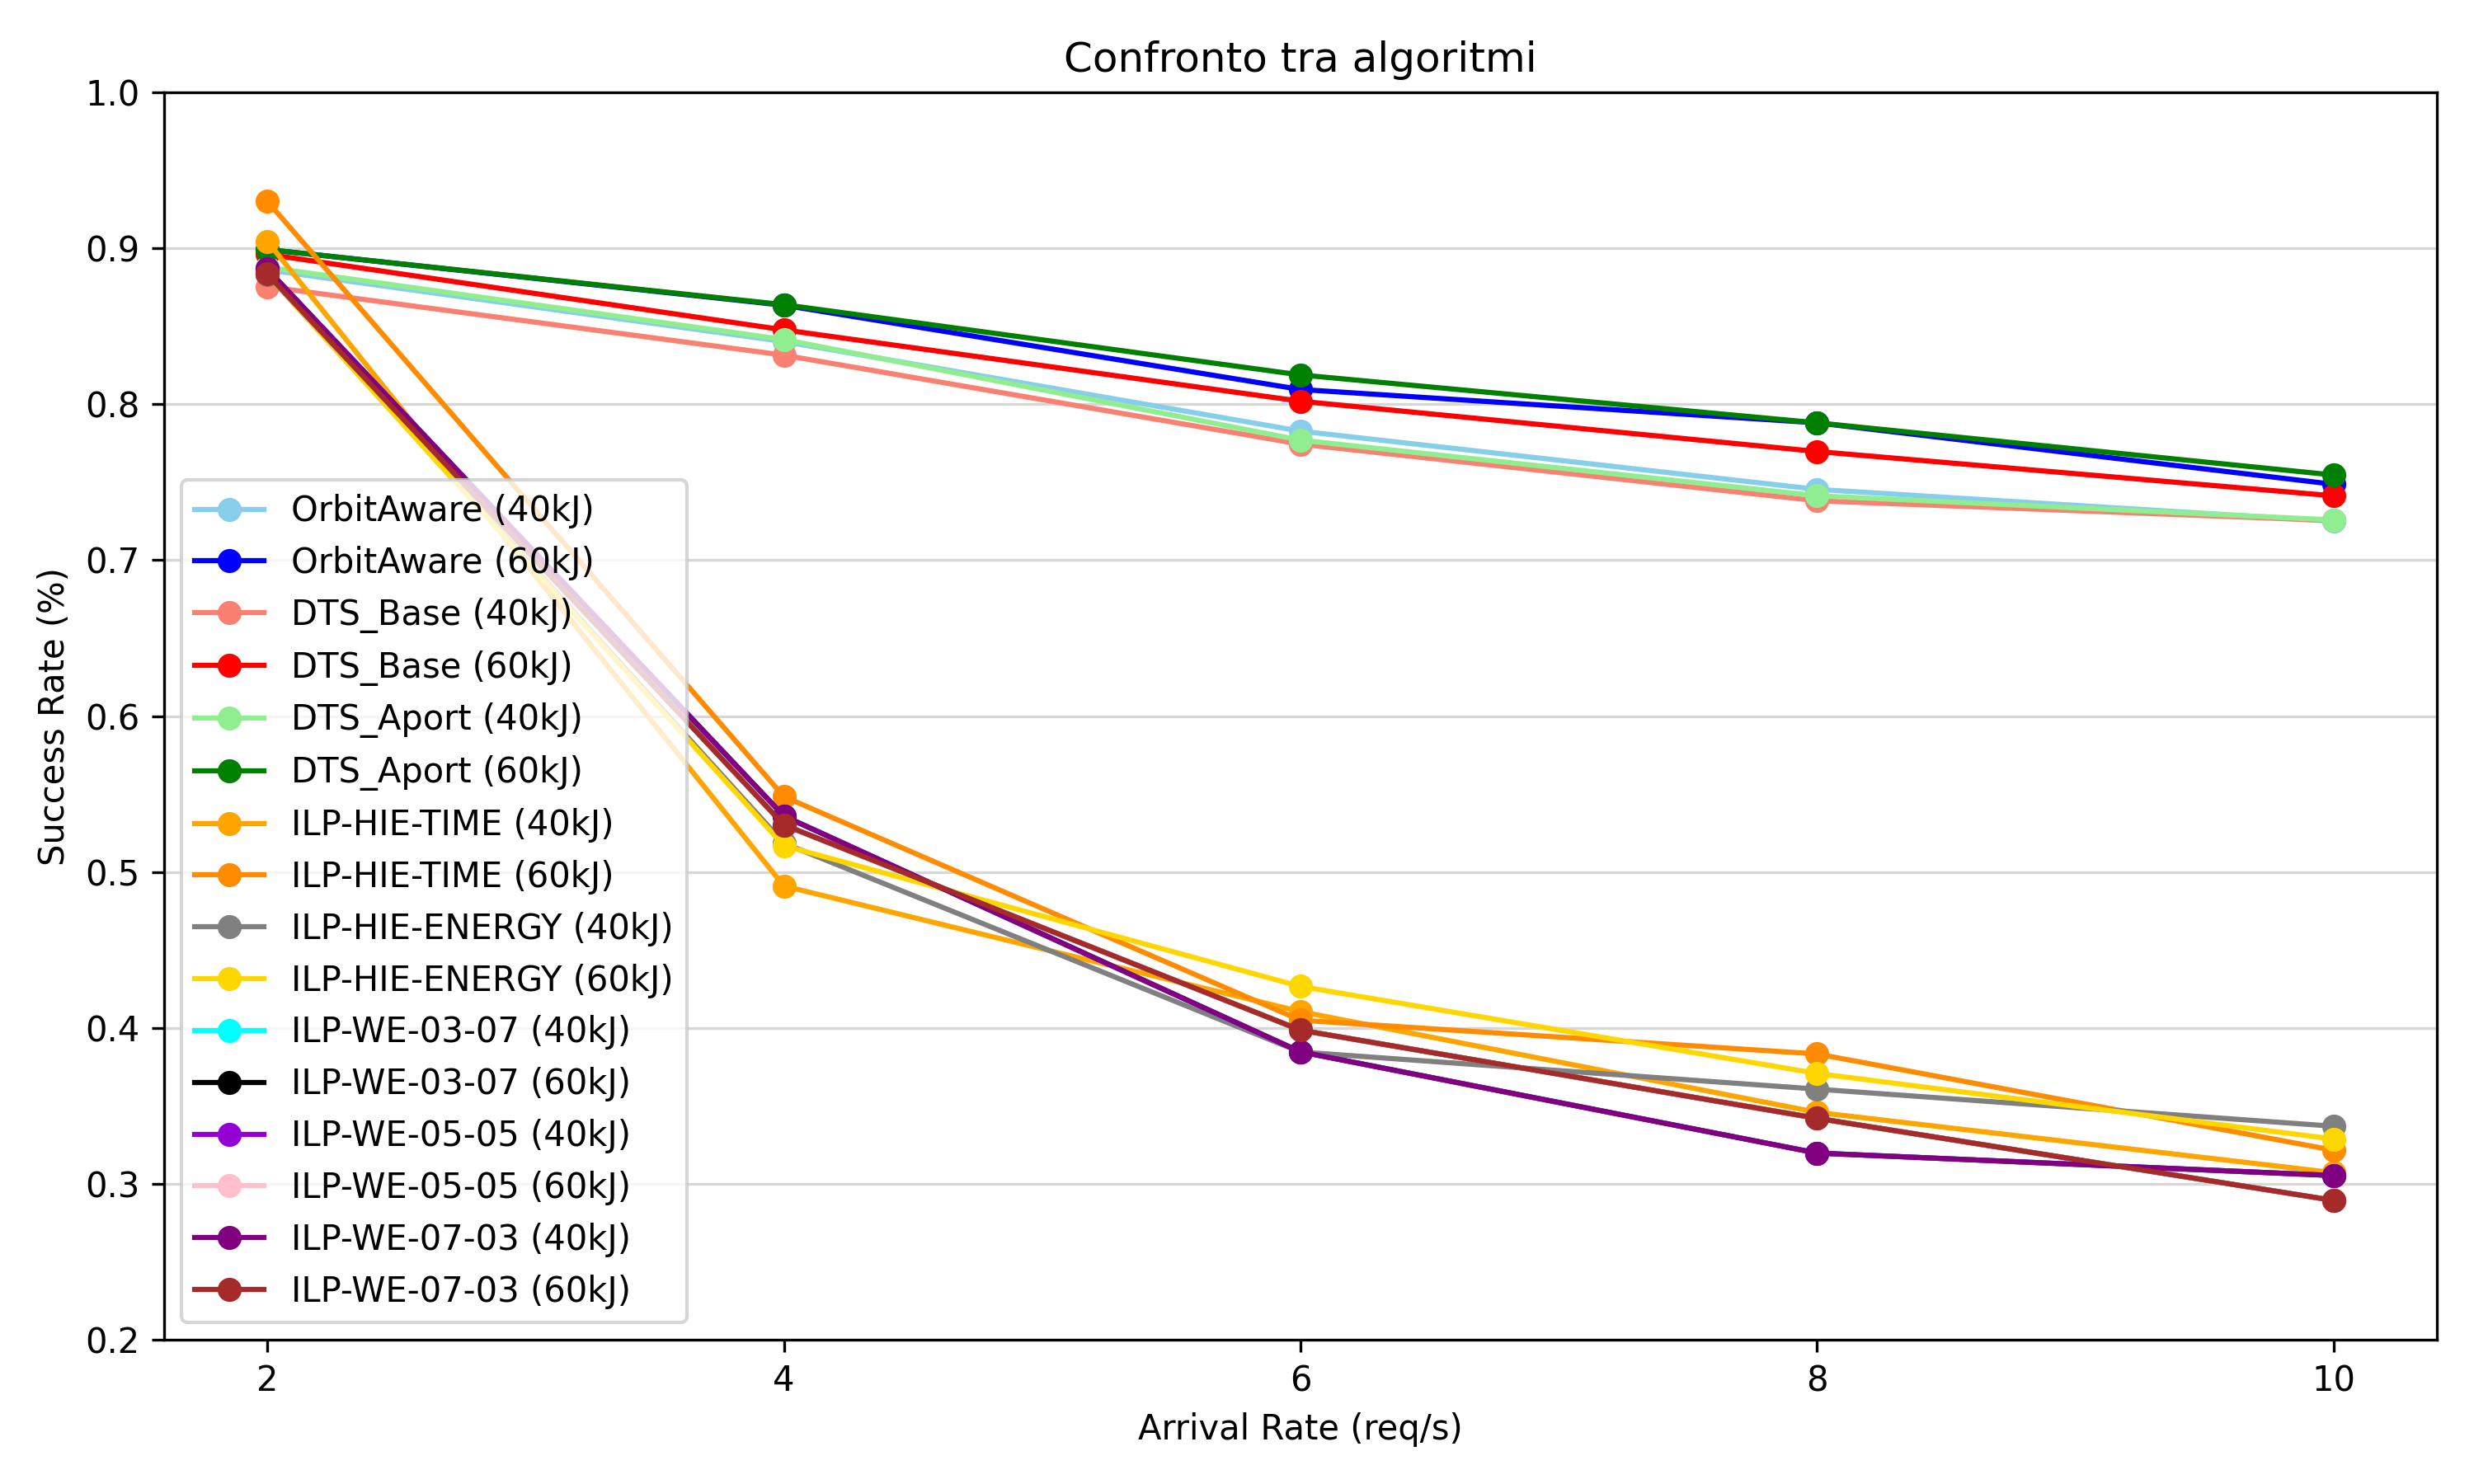
\includegraphics[width=\textwidth,height=0.32\textheight,keepaspectratio]{confronto_algo.png}
        \caption{Success rate al variare del arrival rate}
        \label{fig:confronto-algo}
    \end{subfigure}
    \hspace{0.02\textwidth}
    \begin{subfigure}[b]{0.70\textwidth}
        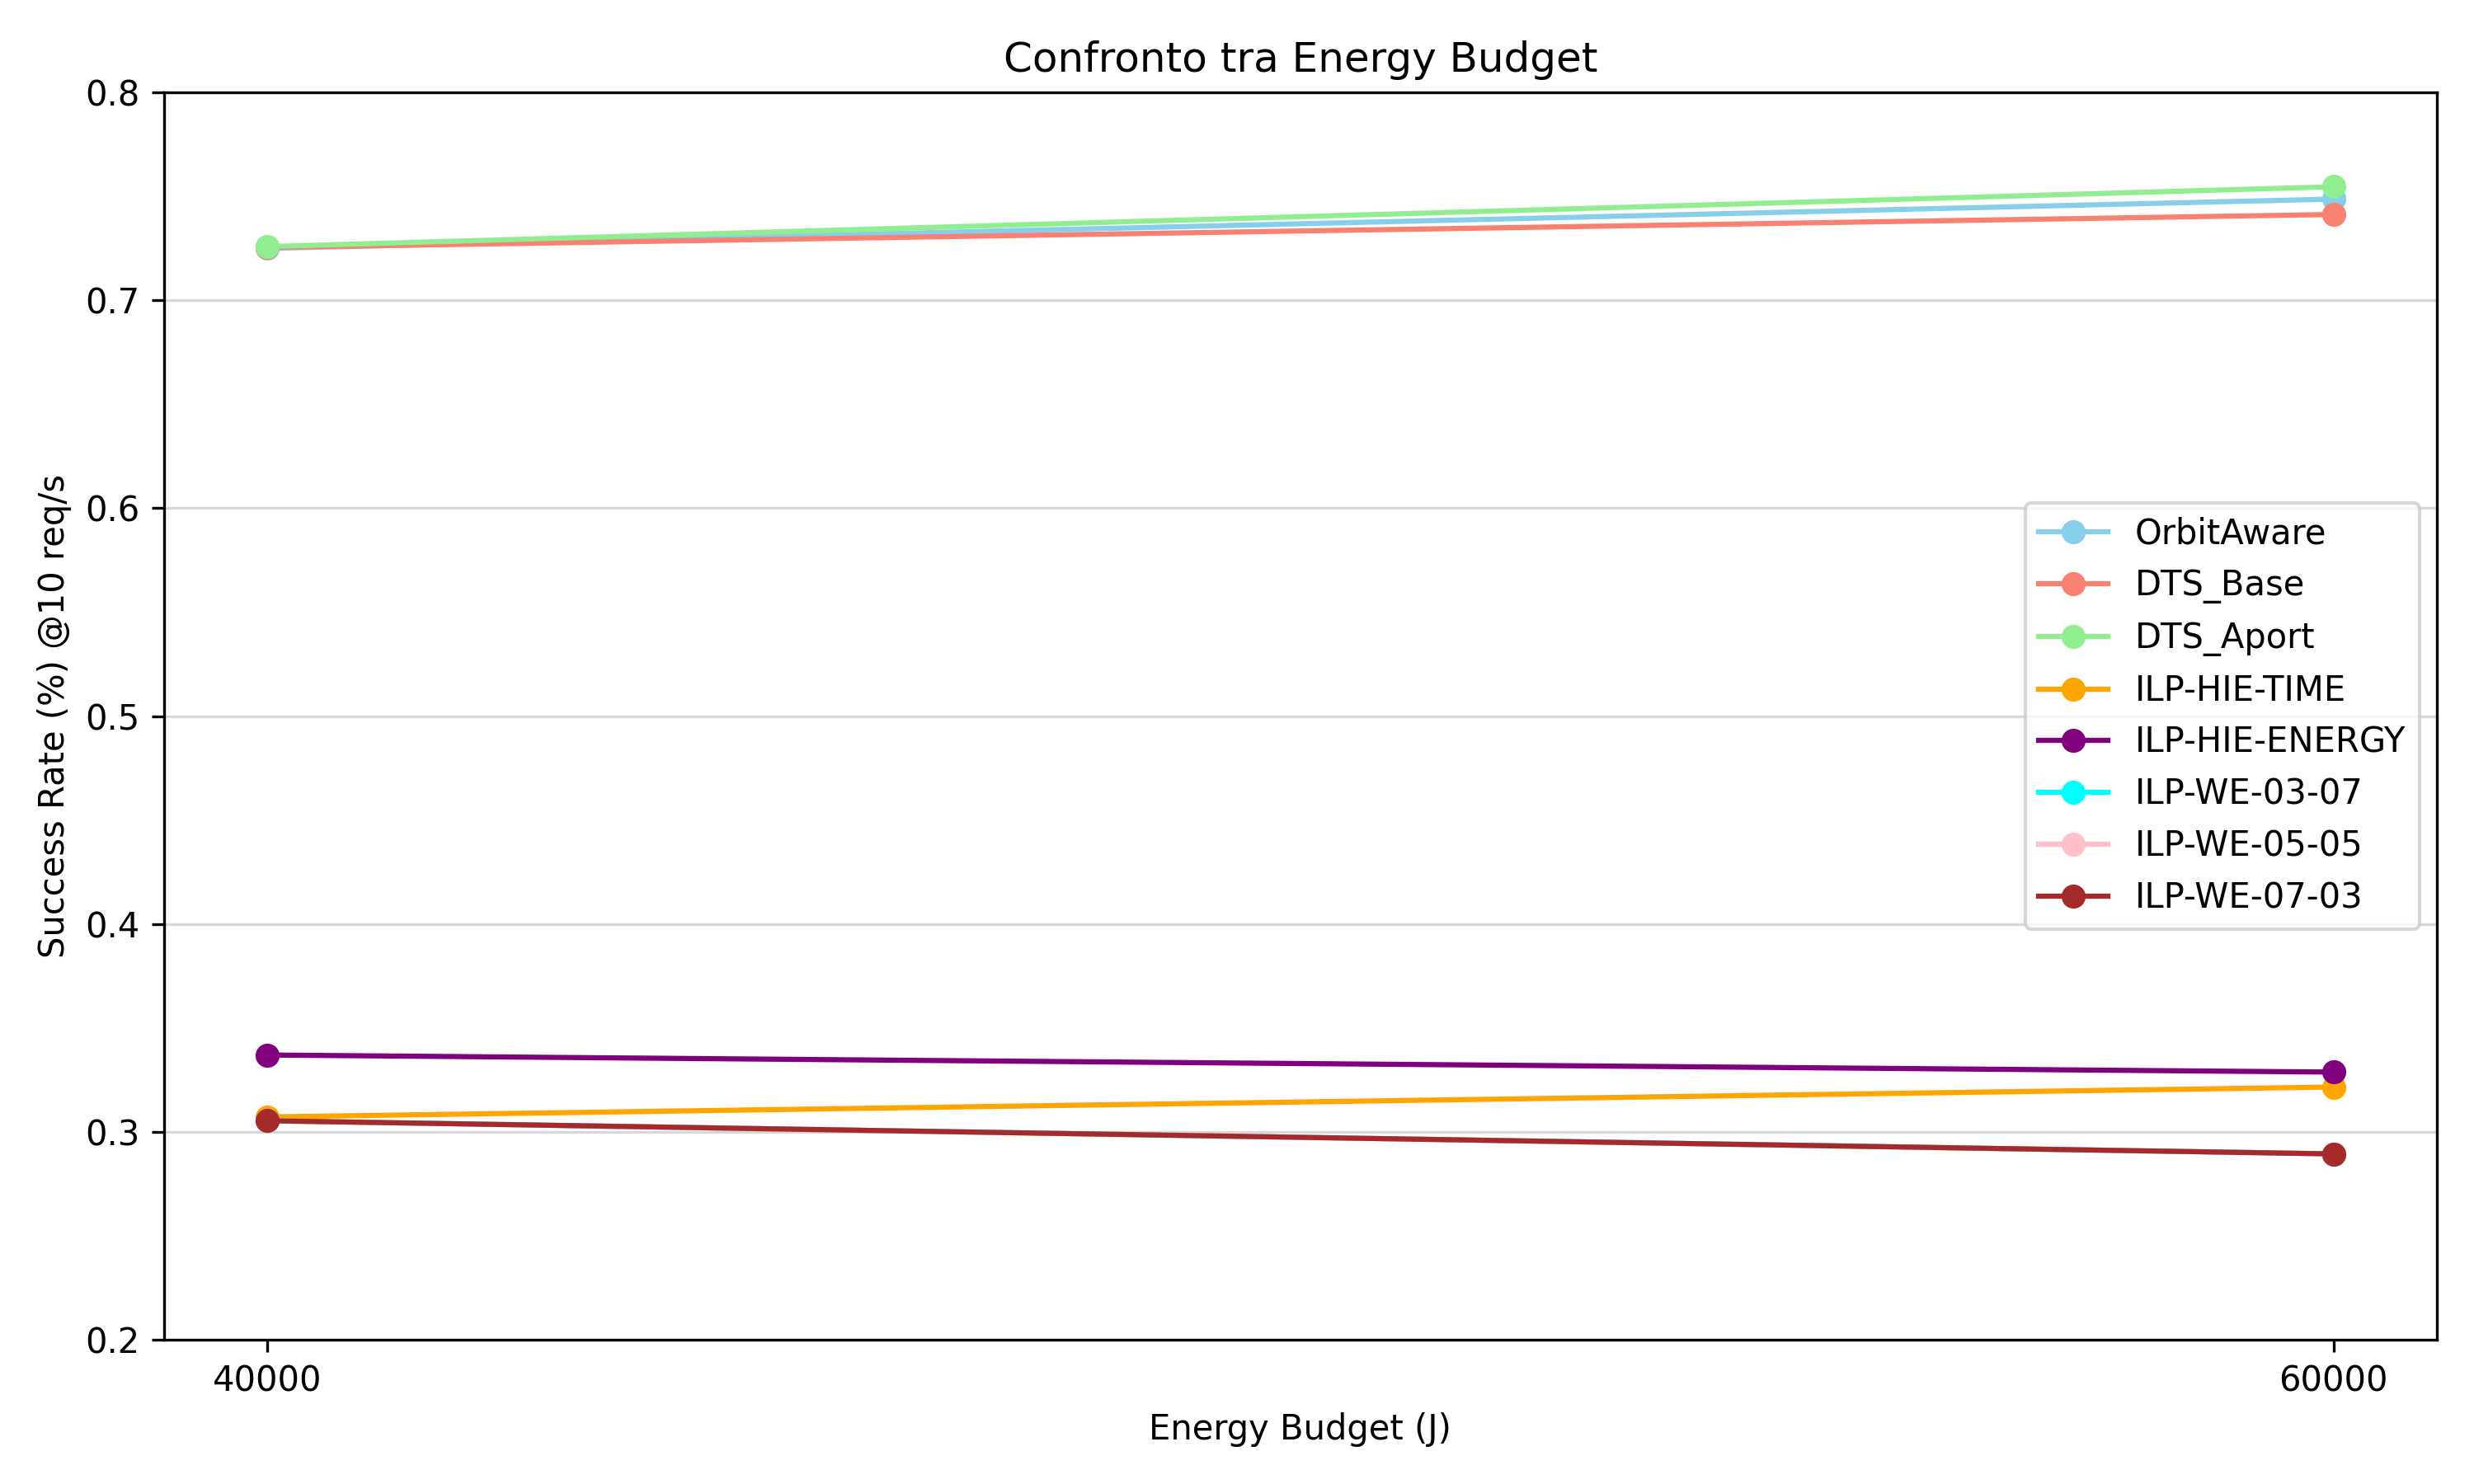
\includegraphics[width=\textwidth,height=0.32\textheight,keepaspectratio]{confronto_budget.png}
        \caption{Success rate al variare del budget energetico}
        \label{fig:conf-buf}
    \end{subfigure}

    \vspace{0.5em}

    % --- Seconda riga ---
    \begin{subfigure}[b]{0.70\textwidth}
        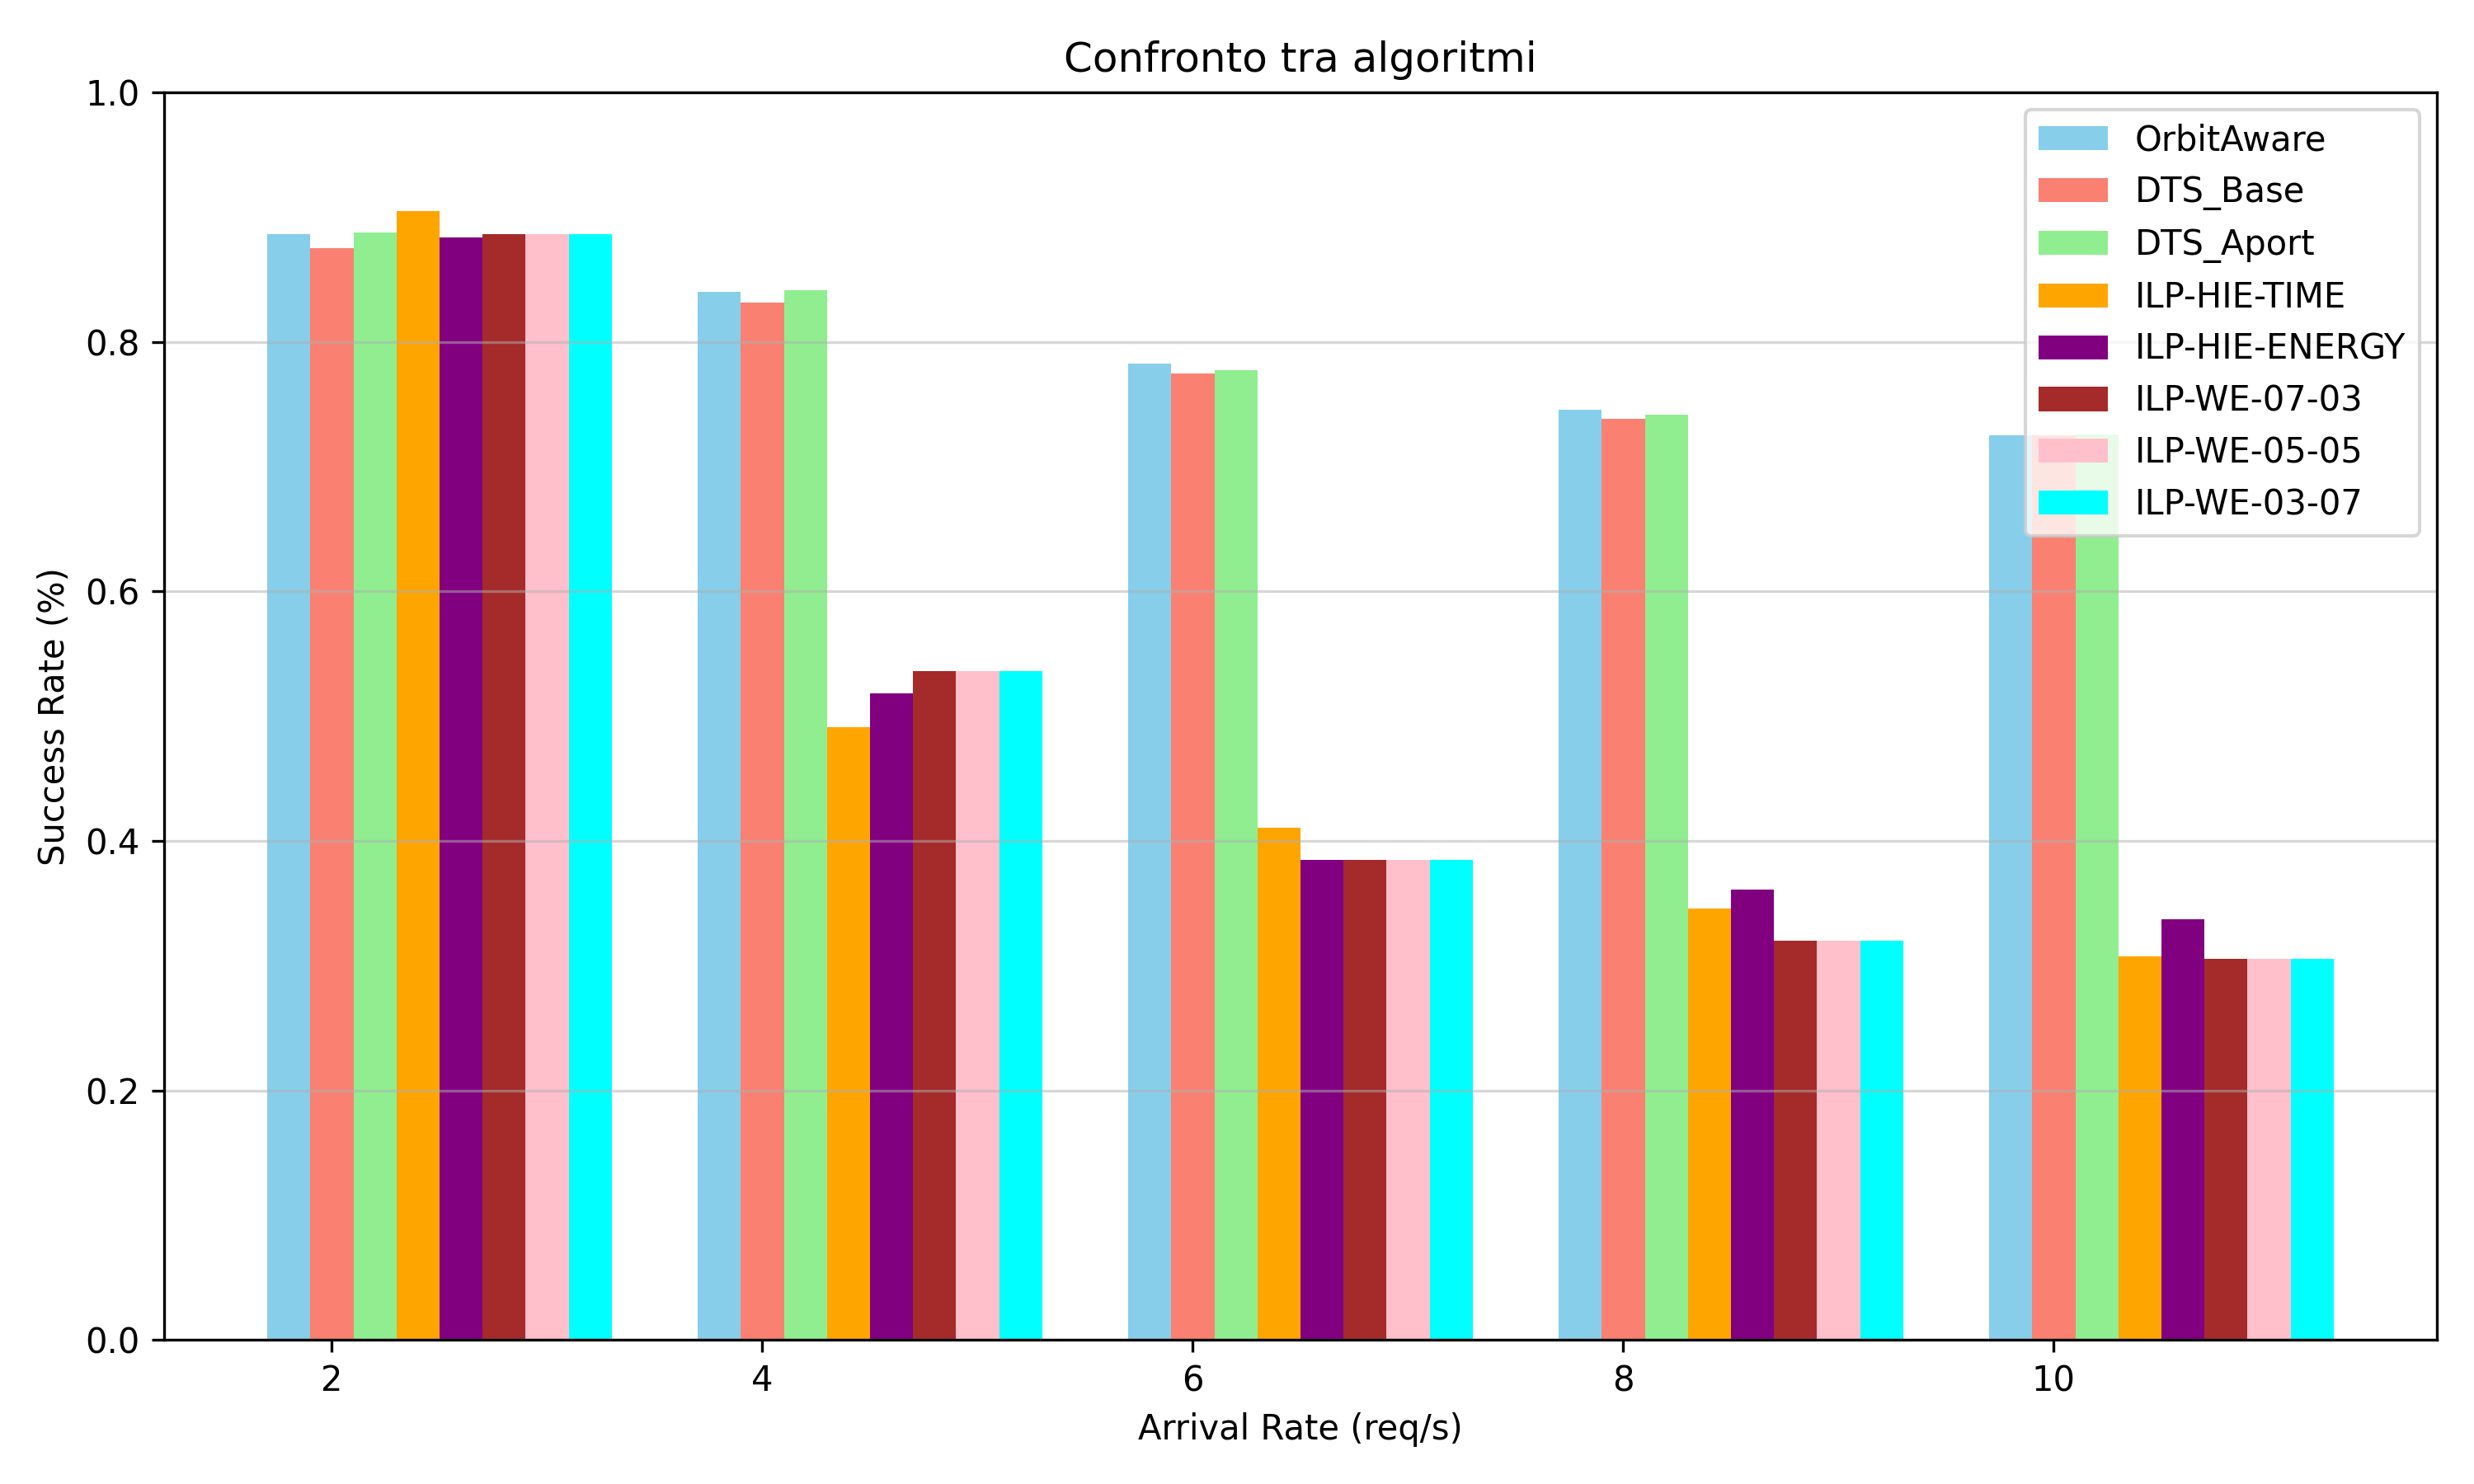
\includegraphics[width=\textwidth,height=0.32\textheight,keepaspectratio]{confronto_algoritmi_40000.png}
        \caption{Success rate con 40\,kJ}
        \label{fig:conf-suc-40}
    \end{subfigure}
    \hspace{0.02\textwidth}
    \begin{subfigure}[b]{0.70\textwidth}
        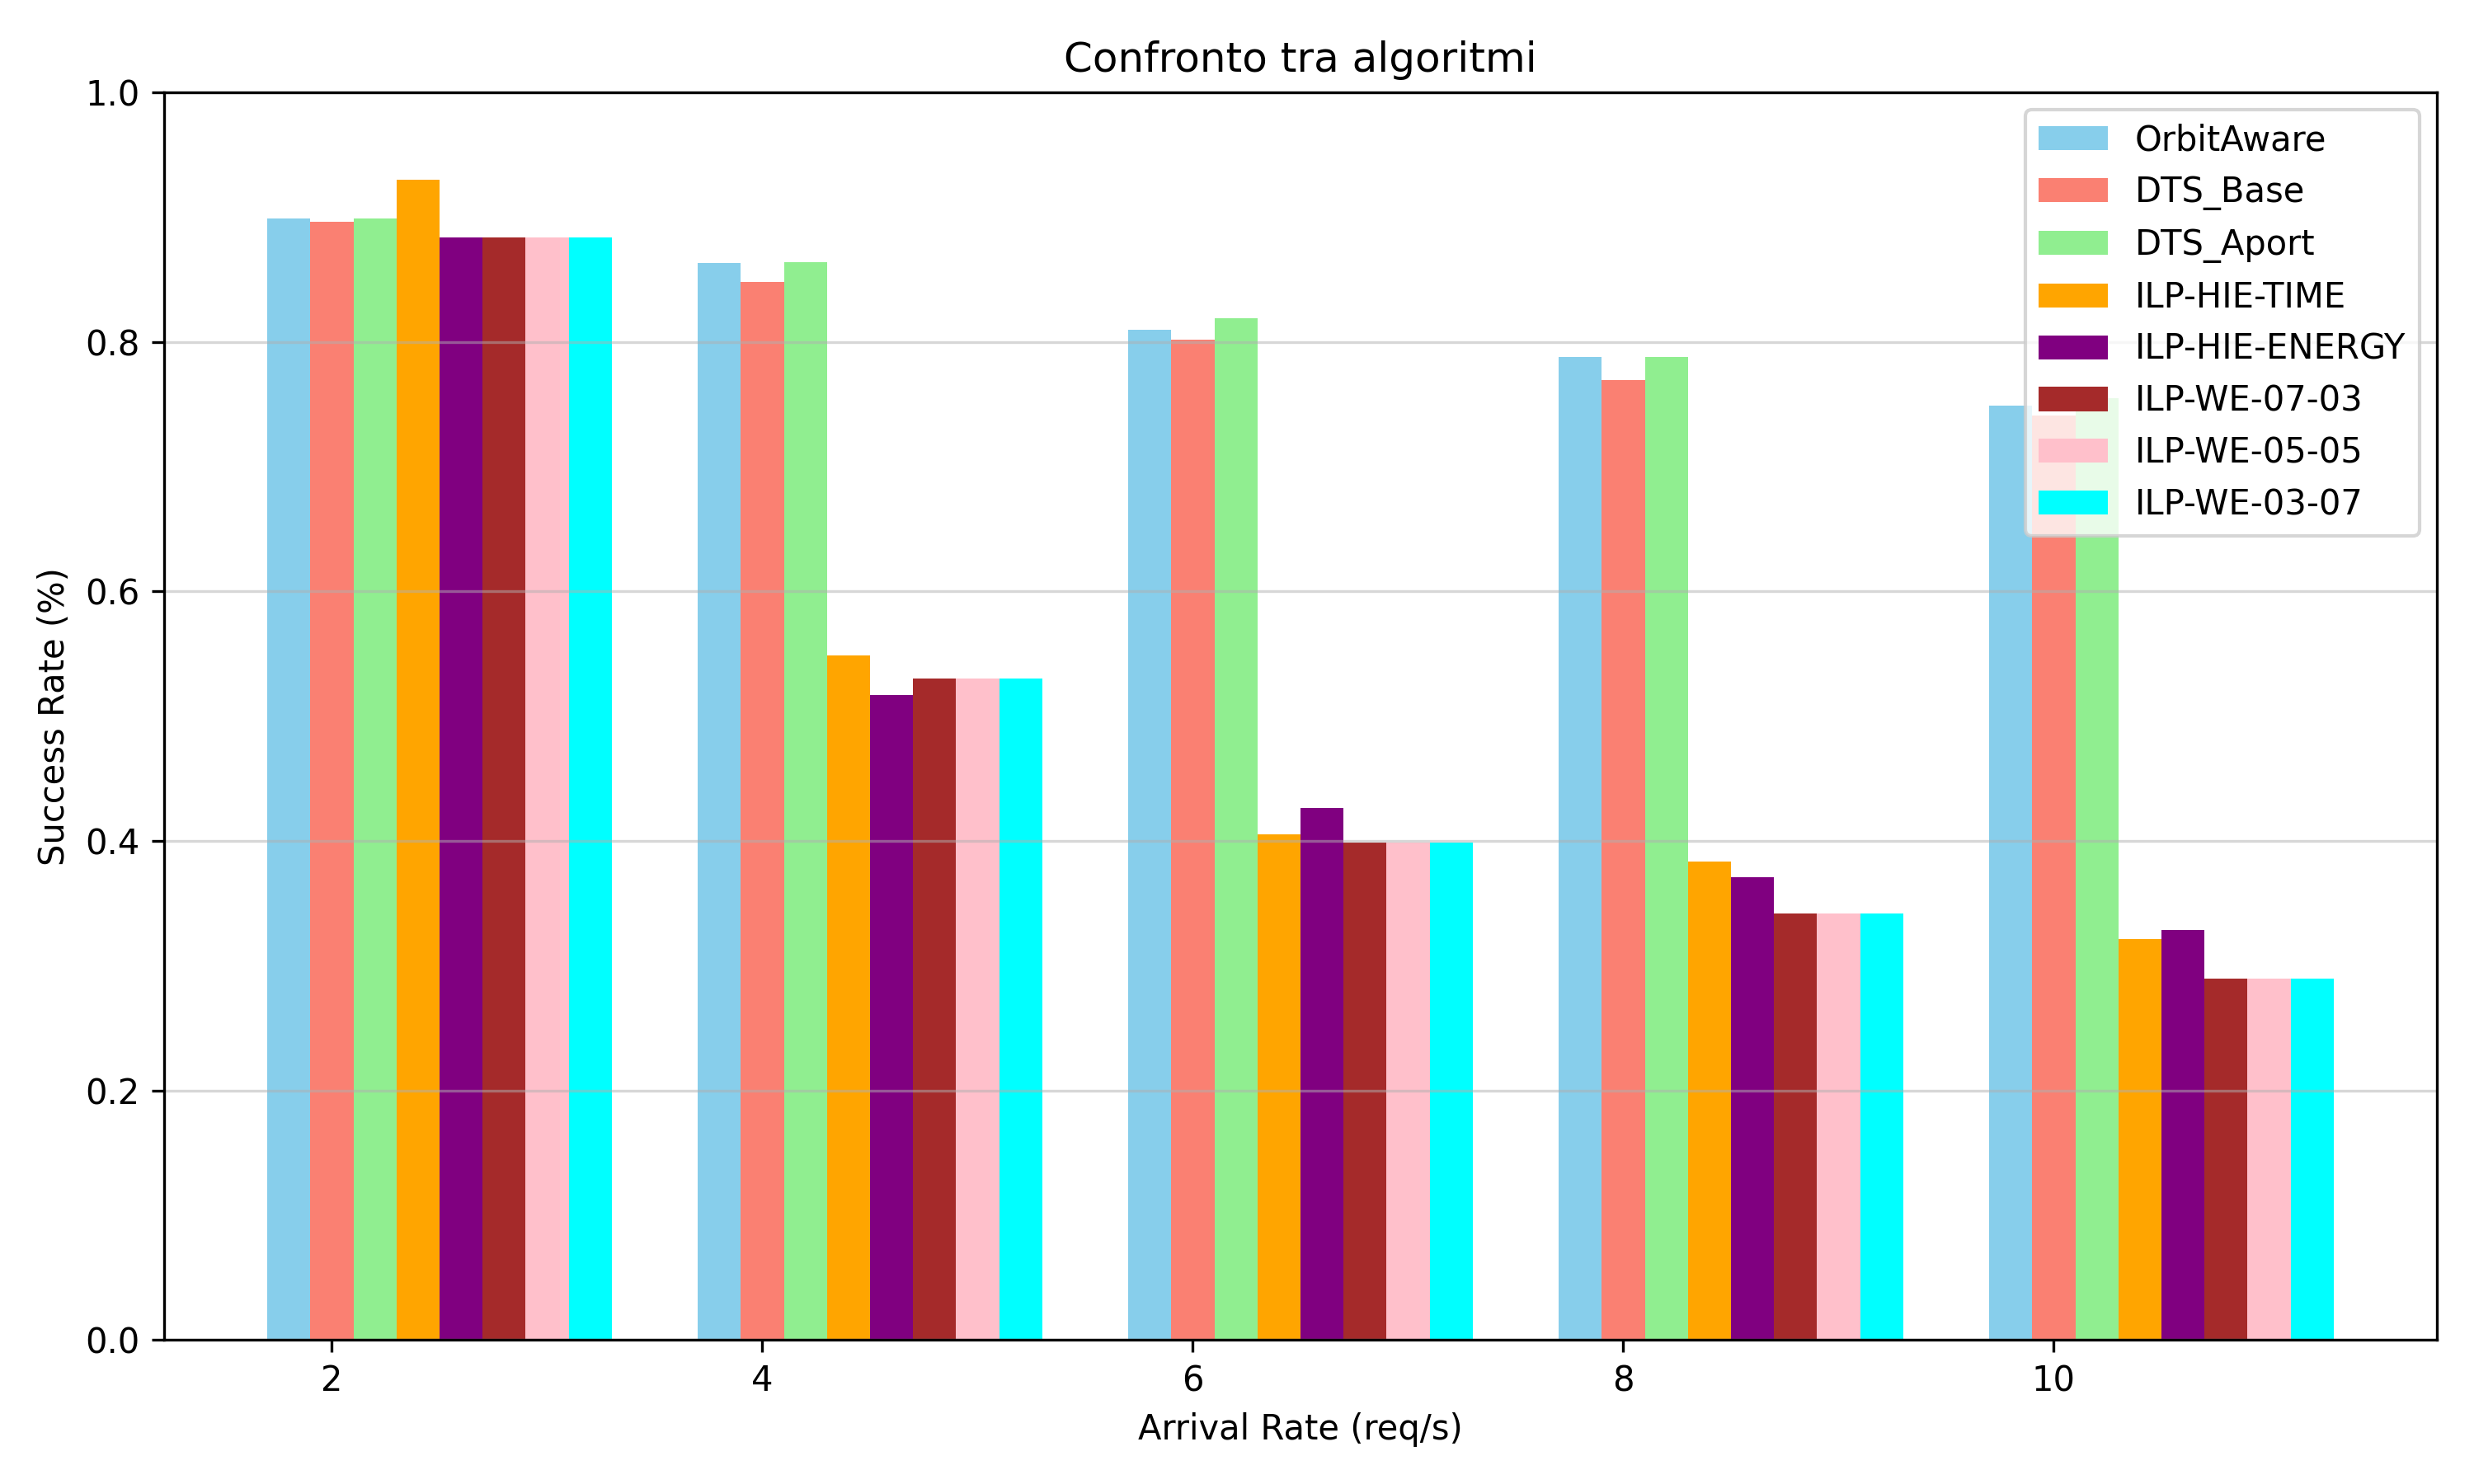
\includegraphics[width=\textwidth,height=0.32\textheight,keepaspectratio]{confronto_algoritmi_60000.png}
        \caption{Success rate con 60\,kJ}
        \label{fig:conf-suc-60}
    \end{subfigure}

    \vspace{0.5em}

    % --- Terza riga ---
    \begin{subfigure}[b]{0.70\textwidth}
        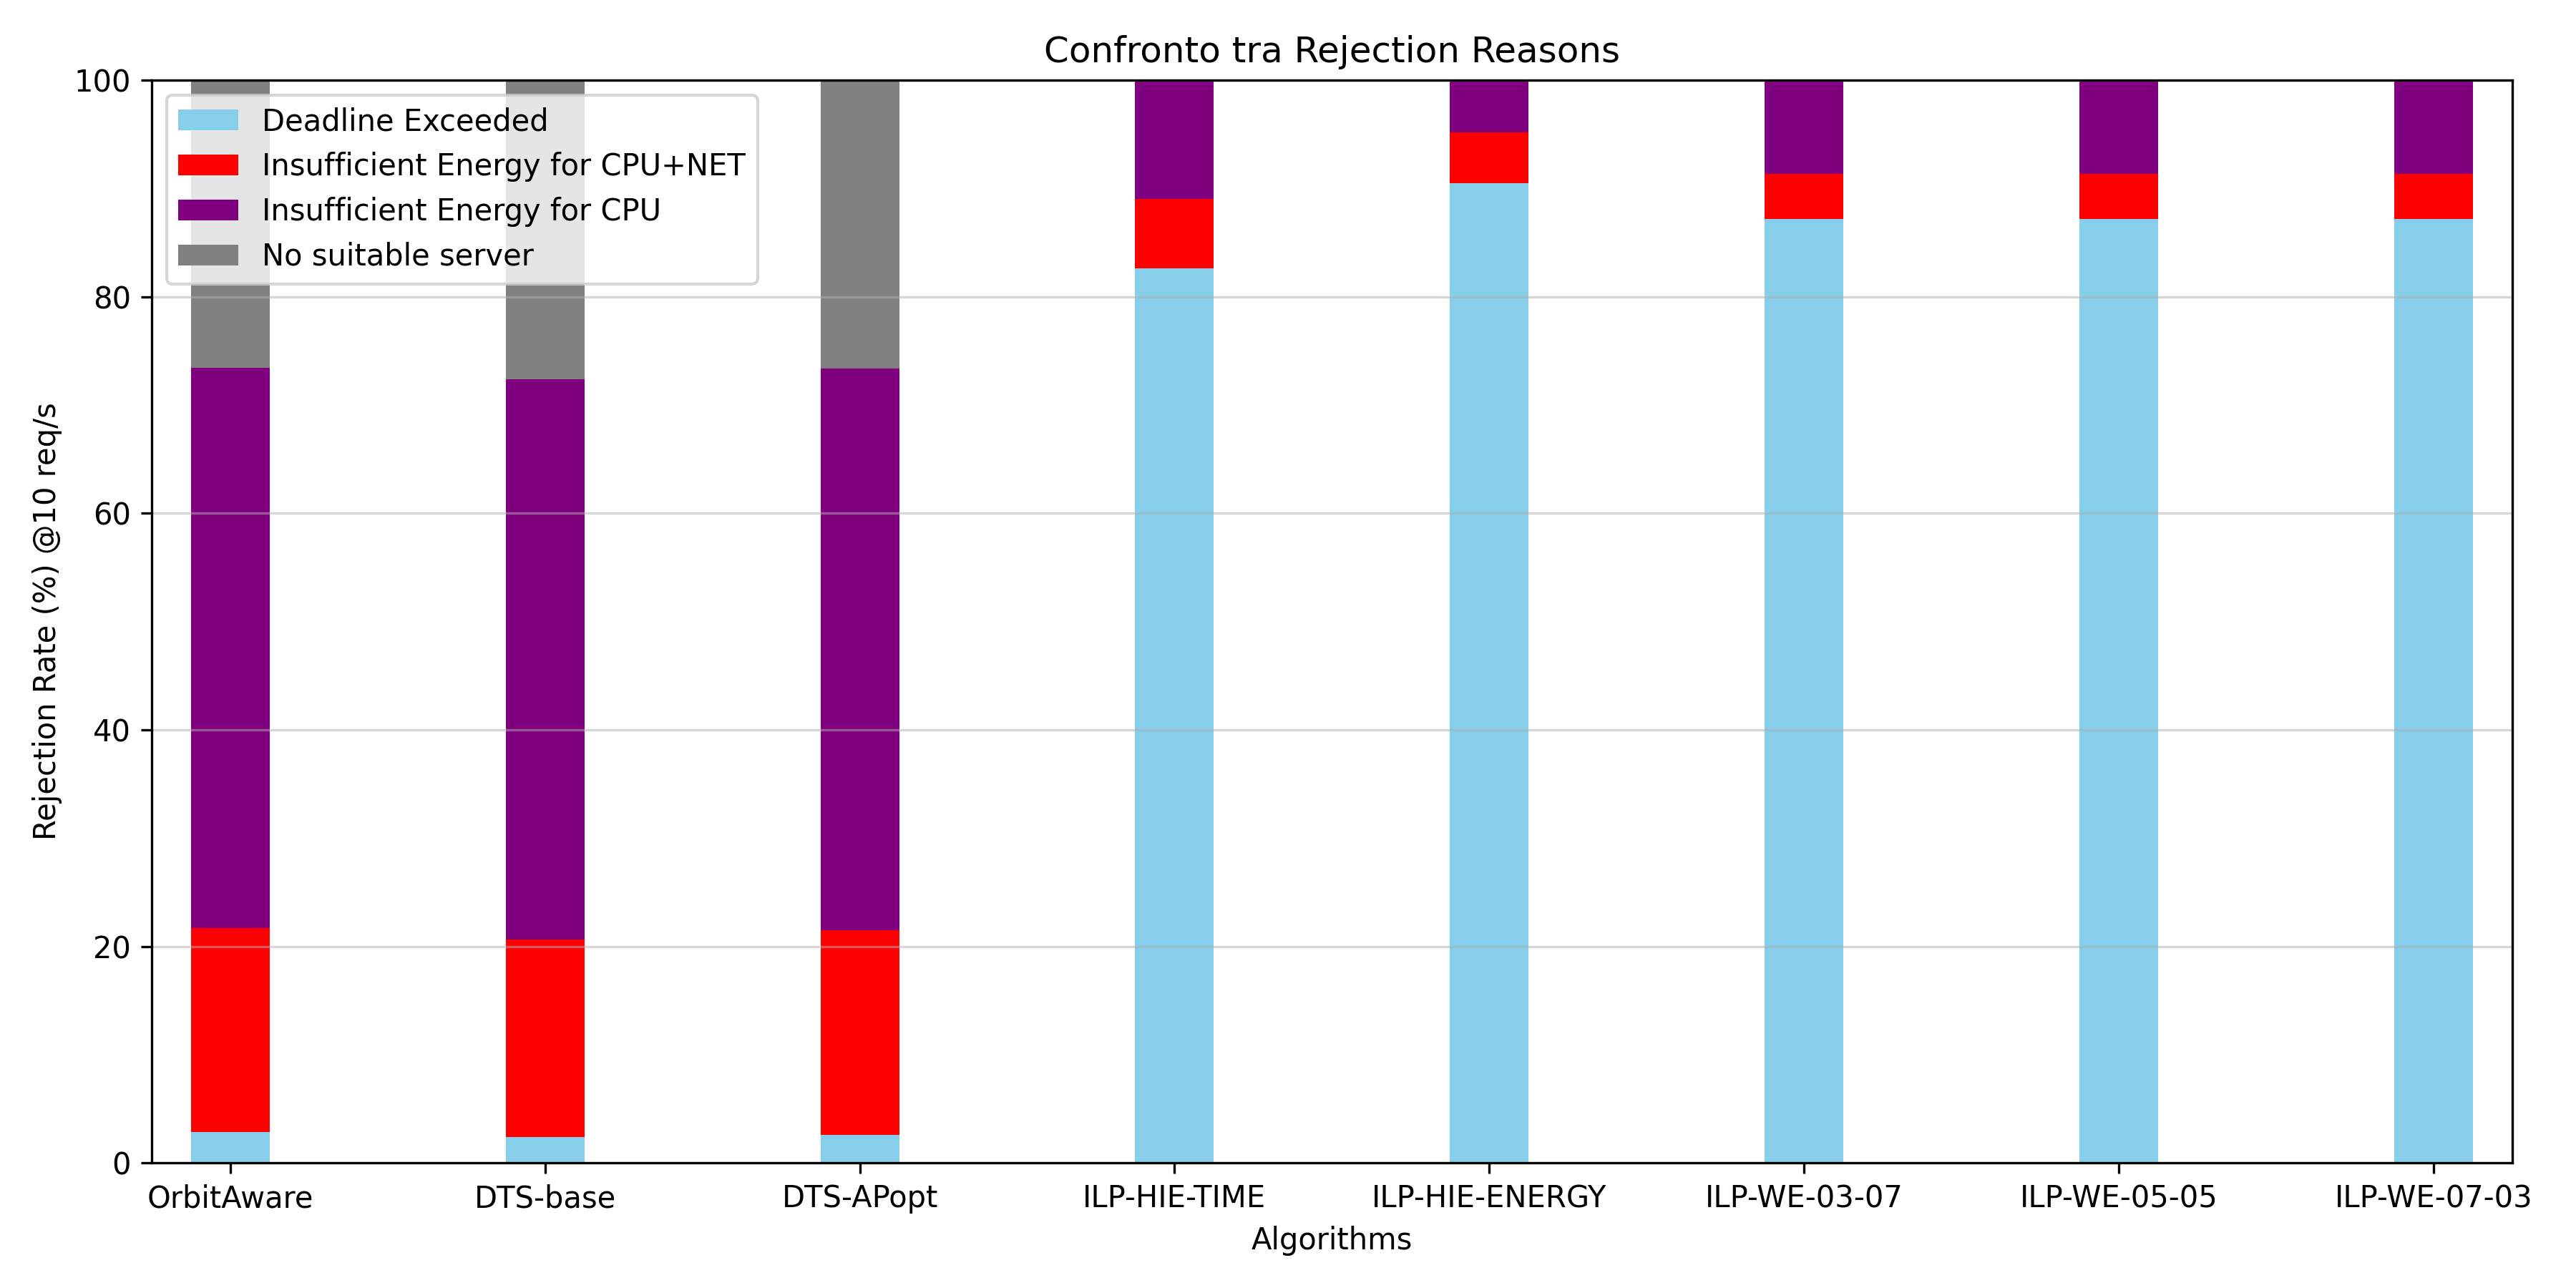
\includegraphics[width=\textwidth,height=0.32\textheight,keepaspectratio]{confronto_rejection_40000.png}
        \caption{Rejection cause con 40\,kJ}
        \label{fig:conf-rej-40}
    \end{subfigure}
    \hspace{0.02\textwidth}
    \begin{subfigure}[b]{0.70\textwidth}
        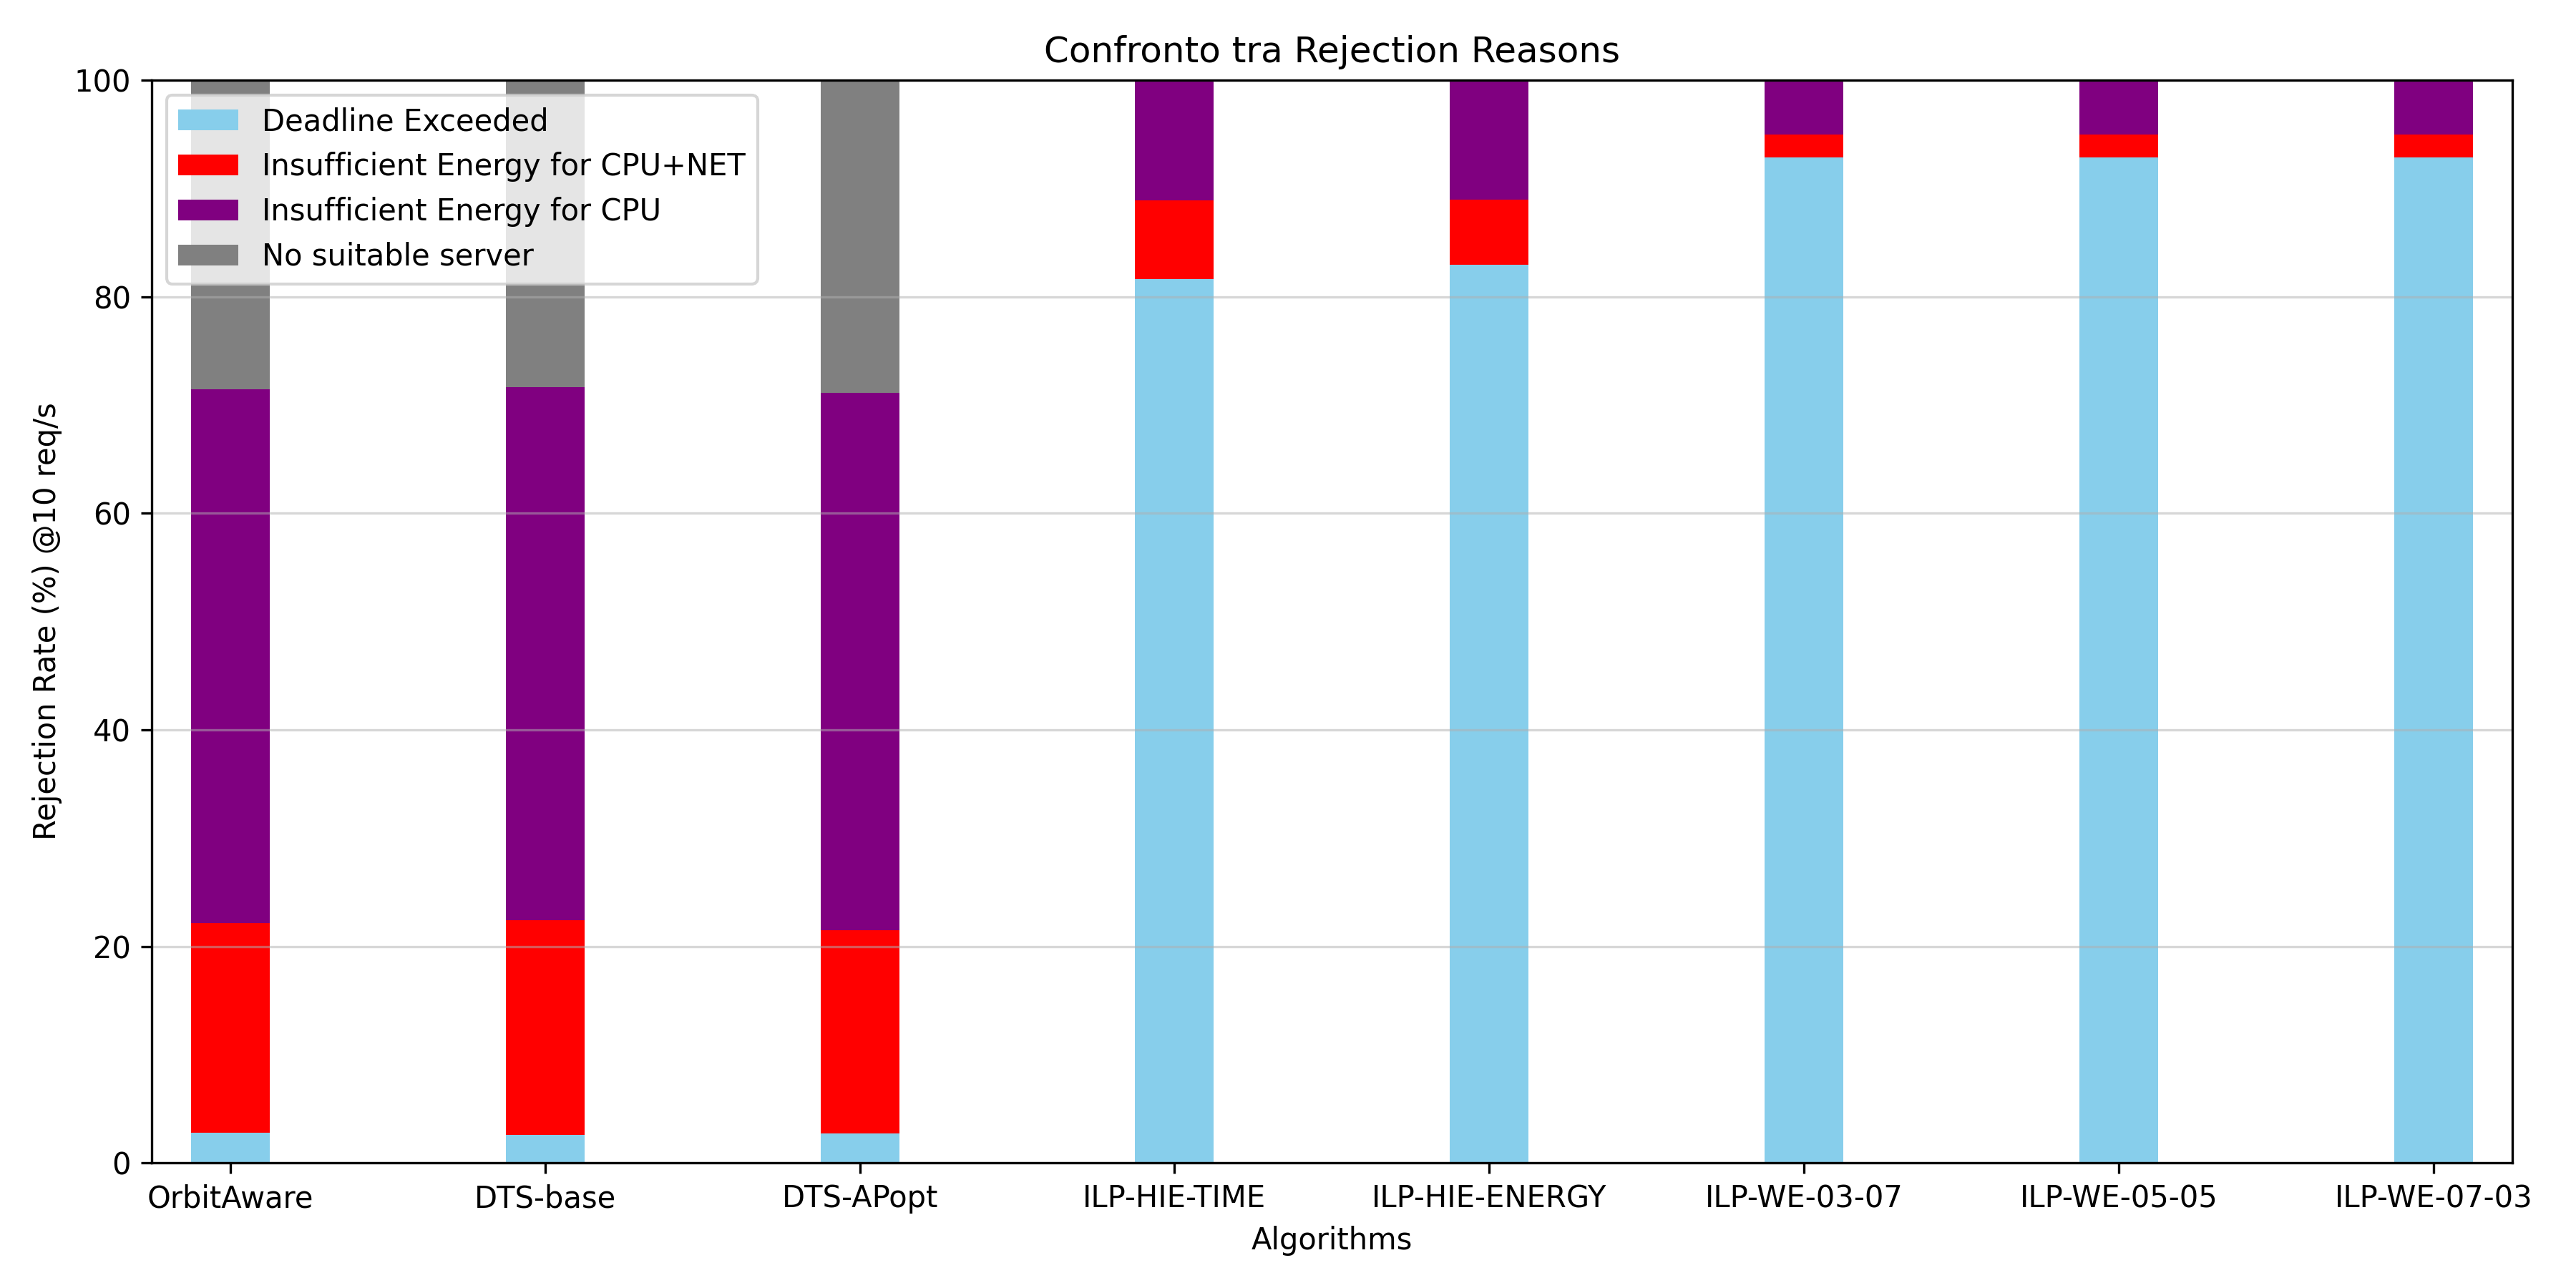
\includegraphics[width=\textwidth,height=0.32\textheight,keepaspectratio]{confronto_rejection_60000.png}
        \caption{Rejection cause con 60\,kJ}
        \label{fig:conf-rej-60}
    \end{subfigure}

    \caption{Grafici dei risultati sperimentali} 
    \label{fig:Grafici}
\end{adjustwidth}
\end{figure}
\FloatBarrier

\section{Conclusione}
In conclusione, l’analisi evidenzia come l’incremento del budget energetico da 40\,kJ a 60\,kJ comporti non solo un miglioramento del \emph{success rate} complessivo, ma anche una significativa riorganizzazione delle cause di rifiuto. In particolare, gli algoritmi ILP mostrano una marcata sensibilità al vincolo di deadline, con dinamiche differenti a seconda della formulazione adottata, mentre gli algoritmi euristici presentano variazioni più distribuite tra vincoli energetici e di disponibilità delle risorse. Ne emerge come la strategia di allocazione influisca in modo determinante sull’equilibrio tra vincoli temporali ed energetici, modificando la natura stessa dei colli di bottiglia del sistema.

\end{document}